% Chapter Template

\chapter{LibVMI\&Volatility Manipulation} % Main chapter title

\label{Chapter7} % Change X to a consecutive number; for referencing this chapter elsewhere, use \ref{ChapterX}

\lhead{Chapter 7. \emph{LibVMI\&Volatility Manipulation}} % Change X to a consecutive number; this is for the header on each page - perhaps a shortened title

%----------------------------------------------------------------------------------------
%	SECTION 1
%----------------------------------------------------------------------------------------

\section{INTRODCTION}
Recall that the objective of this internship derives from a predication made by Pfoh in his doctoral thesis in chapter 6 
Derivative Method \cite{Reference7}: These methods (Derivative method) allow one to track network connections on a per-process
basis in a completely guest operating system agnostic manner.

Frankly, a Virtual Machine Introspection application VMWall \cite{Reference2} has implemented almost the similar functionality. 
However, VMWall’s implementation is based on delivery pattern, thus it has a narrow set of operating system support and requires
some preliminary configuration files to work. All above characteristics hinder wide application of this kind of VMI application.
Therefore, what Pfoh has declared actually attract my attention is the capacity presented by his derivative method to achieve
the same functionality but in a “completely guest operating system agnostic manner”.

To implement his claim, this task could be naturally treated from two plans: network plan and process plan. 
With regard to network plan, Pfoh gives the theoretical groundwork about his predication: All guests I/O activities, 
including network traffic, have to rely on the hypervisor. In other words, performing such network traffic monitoring is a 
matter of tapping into the virtual I/O device within the hypervisor and interpreting the data. Thus, it is not difficult 
to get to know network-related information such as the source/destination IP address, source/destination port number, 
for each network connection. Then we consider the identification of processes in a running guest. According to him, all 
running processes could be identified and represented uniquely by its corresponding CR3 register value. Assuming that 
network plan for implementation of his claim is finished and the running process list is obtained, it remains how to find 
and associate the corresponding process information (represented by CR3 value) according to obtained network information 
(represented by source/destination IP address and port). For VMWall, the key attribute to do this association is connection
port number. For a derivative method, still back to Pfoh’s work, he has stated that one could identify a unique process by 
inspecting CR3 register. Unfortunately, he didn’t expatiate how to associate CR3 register value and network information. 
We don’t know which attribute is shared by network connection and CR3 register. In fact, this is the most important part in 
the course of implementing Pfoh’s predication.

Stuck with this step for longtime, in the meantime, I have tried to explore if the system call (such as read(), wirte(), 
socket()) related to network I/O, or I/O interrupt could associate network connection and a CR3-represented process. 
Due to the lack of documentation in this domain, I have none significate discovery. Hence I tried to think in our objective
in another perspective. Firstly, the reason why we prefer derivative method is its OS-agnostic property, if some powerful 
VMI tools of out-of-band method could provide the same or similar OS-agnostic property, we could give it a try. After all, 
out-of-band VMI research domain is much more active than derivative method and therefore provides more powerful tools. 
Secondly, our exploration about derivative method is to watch its possible contribution to monitoring task. In this angle, 
derivative method is inherently limited compared to delivery method, because derivative method works in low-level and could
not get high-level information (Obviously, high-level information is usually related to operating system kernel data 
structure). Thirdly, we could try to firstly implement a network connection monitor in out-of-band manner and may get some 
inspiration for a derivative method implementation. In addition, this delivery method implementation could be used as a 
reference for future derivative method implementation.

During the searching online, I have noticed that currently leveraging forensic memory analysis tools, also known as FMA, is 
a popular tendency in Virtual Machine Introspection application development \cite{Reference33}. The remains of this section is 
aimed to record the exploration of how to leverage FMA tool such as Volatility with VMI tools such as LibVMI for running virtual 
machine.

\section{FORENSIC MEMORY ANALYSIS TOOL}
Forensic Memory Analysis is the science of using a memory image to determine information about running programs, the operating system
, and the overall state of a computer \cite{Reference34}. Because the analysis is highly dependent on the operating system, it has 
been divided into the following categories:
\begin{itemize}
    \item Linux Memory Analysis
    \item Mac OS X Memory Analysis
    \item Windows Memory Analysis
\end{itemize}
Similar with Virtual Machine Introspection, the FMA community is also faced with the semantic gap problem to extract 
forensically relevant information from dumps of physical memory. The only difference between VMI and FMA regarding 
semantic gap lies in that VMI is used to monitor a running guest’s memory (dynamic file) while FMA initially is used to 
analyze memory dump file (static file). Figure \ref{fig:Comparison of VMI and FMA} shows the relationship between FMA and VMI.

Up to now, FMA community has made plenty achievements to mitigate semantic gap. Many excellent FMA tools, such as Volatility framework, 
are available. The following figure shows the comparison between the famous VMI tool LibVMI and Volatility. Since after many years 
developments, Volatility has a wide set of memory analysis support, from Android to Mac, from Linux to Windows. Hence, leveraging this 
characteristic, it is possible to create an OS-agnostic VMI application, if we have some approaches to make Volatility treat virtual 
machine’s memory as a recognizable file. Fortunately, LibVMI, a VMI framework based on out-of-band method, has developed a python-wrapper
which allows Volatility functioning for a running guest.

\begin{figure}[htbp]
	\centering
		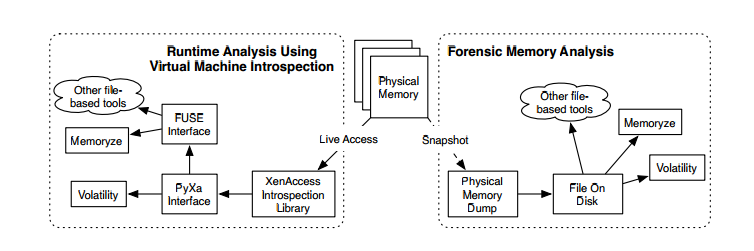
\includegraphics[width=14cm, height= 8cm ]{Figures/Figure20.png}
	\caption[Comparison of VMI and FMA]{Comparison of VMI and FMA \cite{Reference3}}
	\label{fig:Comparison of VMI and FMA}
\end{figure}

\section{INSTALLATION LIBVMI AND VOLATILITY IN KVM}
This section will introduce how to install LibVMI\&Volatility in Ubuntu14.04, where KVM virtualization platform has been 
established with success. With regard to how to establish KVM platform in Ubuntu14.04, this link 
http://adywp.blogs.unhas.ac.id/2014/05/installing-kvm-on-ubuntu-14-04/ is strongly recommended.

It is worth to mentioning that the libvirt library, installed by Ubuntu's package manager (for example by apt-get), 
does not support QMP command, which is necessary for QEMU emulator to access directly target guest's physical memory. 
Similarly, QEMU utility installed by default does not provide functions to access virtual machine's memory. Hence, 
to use LibVMI in KVM platform, the first step is to get respectively source codes for libvirt and QEMU, modify QEMU to add 
VM physical memory access code and install these utilities from source code.

To get libvirt source code, open a terminal and change into your destination directory (in our case, we plan to arrange 
all source codes required under a directory called "libvmi") and issue this command in a terminal:
\shellcmd{
		mkdir ~/libvmi \\
\#		cd ~/libvmi \\
\#		wget http://libvirt.org/sources/libvirt-1.2.6.tar.gz \\
\#		tar zxvf libvirt-1.2.6.tar.gz \\
\#		cd libvirt-1.2.6
}
When compiling and installing libvirt from source code, notice that an older version (version 1.2.2) has been already 
installed under path /usr/bin, to avoid any possible confusion, we need to update libvirt by overriding the old one:
\shellcmd{
		./autogen.sh \\
\#		./configure --prefix=/usr --localstatedir=/var --sysconfdir=/etc \\
\#		make \\
\#		sudo make install\\
\#		sudo ldconfig
}
Then, do not forget to modify libvirt configuration file and restart libvrit daemon. Modify /etc/libvirt/libvirtd.conf, uncomment this line:
\shellcmd{auth\_unix\_rw = “none”}
To restart libvirtd, type the following commands:
\shellcmd{
			sudo /etc/init.d/libvirt-bin stop \\
\#			sudo /etc/init.d/libvirt-bin start			
}
In term of QEMU, we need to firstly know why and how to modify its source code. What the patch actually does is to use 
Qemu Machine Protocol (QMP) mechanism for LibVMI to pass the GPA (Guest Physical Address), and call the internal function 
"cpu\_physical\_memory\_map" located in qemu/exec.c in Qemu, and finally get the mapped HVA (Host Virtual Address) back. 
More details about how to write a patch for a certain version of QEMU are available in this link:
\url{http://ytliu.info/blog/2014/03/27/kvm-support-in-libvmi}. Given that a QEMU patch for QEMU 1.6 is provided, we use git
to clone branch 1.6 version of QEMU:
\shellcmd{
mkdir ~/libvmi/qemu-stable-1.6 \\
\#\indent\indent\texttt{cd qemu-stable-1.6} \\
\#\indent\indent\texttt{git init} \\
\#\indent\indent\texttt{git remote add -t state-1.6 -f origin https://github.com/qemu/qemu.git} \\
\#\indent\indent\texttt{git checkout stable-1.6}
}
Supposing that the path of patch file for QEMU 1.6 is ~/libvmi/kvm-1.6-patch.patch, to patch QEMU, issue this command:
\shellcmd{
		patch -p1 < ../kvm-1.6-patch.patch \\
\#		./configure --prefix=/usr --target-list="386-softmmu x86\_64-softmmu"		
}
By default (without –target-list option), ‘configure’ will prepare many machine type emulator, and it takes long time to compile.
\shellcmd{
		make \\
\#		sudo make install
}
In addition, to assure the functioning of LibVMI, all the following additional packages are required to be installed:
\shellcmd{
sudo apt-get install zlib1g-dev libglib2.0-dev libpixman-1-dev libfdt-dev libtool libsdl1.2-dev \\
\#		sudo apt-get install libbison-dev flex libyajl-dev check autopoint python-dev libxslt1-dev xsltproc \\
\#		sudo apt-get install libdevmapper-dev libpciaccess-dev libnl-dev w3c-dtd-xhtml libjansson-dev libfuse-dev
}
Now all prerequisites works are done to install LibVMI. To get its source code, type this command:
\shellcmd{
cd ~/libvmi \\
\#		git clone git://github.com/bdpayne/libvmi.git
}
Then change into LibVMI directory
\shellcmd{
cd libvmi
\#		./autogen.sh \\
\#		./configure \\
\#		make \\
\#		sudo make install \\
\#		sudo ldconfig
}
If all required packages are present in system, after running. /configure command, we should the output shown in Figure 
\ref{fig:Output of ./configure for LibVMI}.
\begin{figure}[htbp]
	\centering
		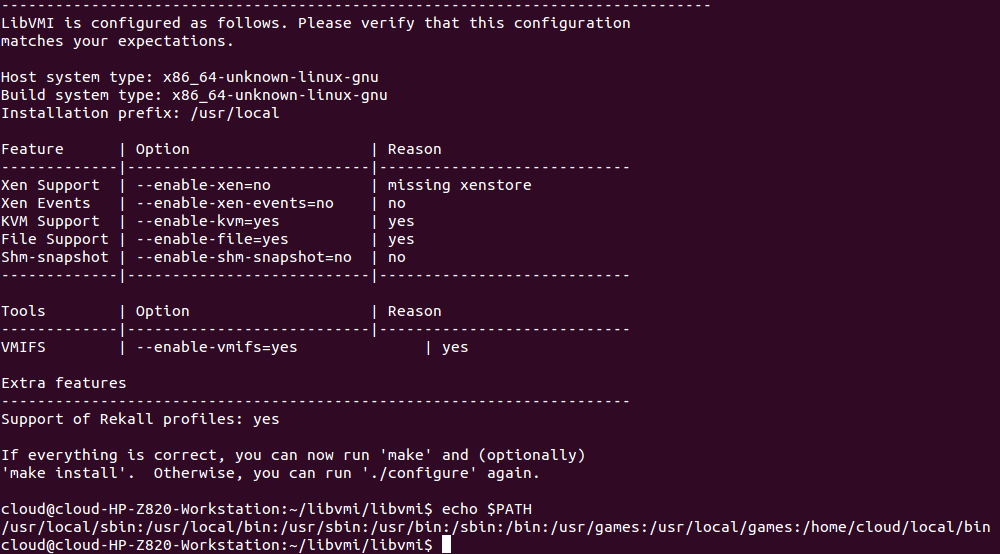
\includegraphics[width=14cm, height= 10cm ]{Figures/Figure21.png}
	\caption[Output of ./configure for LibVMI]{Output of ./configure for LibVMI}
	\label{fig:Output of ./configure for LibVMI}
\end{figure}

LibVMI will be installed in path /usr/local/bin. It is worth to mentioning that after update of QEMU and libvirt, 
some KVM's virtual machines, which are installed under the help of older libvirt version, will encounter some problems 
to start. This is caused by the name convention difference in virtual machine XML configuration file.

After modifying target guest virtual machine's configuration, reload it to take effect
\shellcmd{sudo service livirt-vin reload}
Then all guests who have problems to start now could work normally as before. To verify the correct installation of 
LibVMI, we need to execute the example "process-list" shipped with LibVMI. This example needs some configuration file 
to work. The details on this file can be read here: \url{https://code.google.com/p/vmitools/wiki/LibVMIInstallation}. In
our situation, we put this configuration "libvmi.conf" under path ~/etc/. The most difficult task to complete the LibVMI 
configuration file is how to get "offset" value for certain kernel data structure. Fortunately, LibVMI has provided 
specific tools for this task.

Ignoring the process of how to edit this file, the following is the part of libvmi.conf:

vm2 \{\\
	ostype = "Linux";\\
	sysmap = "/home/cloud/etc/System.map-2.6.32-38-generic";\\
	linux\_name = 0x30c;\\
	linux\_tasks = 0x1d8;\\
	linux\_mm = 0x1f4;\\
	linux\_pid = 0x214;\\
	linux\_pgd = 0x28;\\
\}

vm1\{
\\
	ostype = "Windows";
\\
    	win\_tasks   = 0x188;
\\
    	win\_pdbase  = 0x28;
\\
   	win\_pid     = 0x180;\\
    	win\_pname   = 0x2e0;\\
\}

Executing the following command, we should see the list of currently running processes inside vm2.
\shellcmd{sudo process-list vm2}
From now on, we could say that LibVMI has been successfully installed in our KVM virtualization platform. LibVMI allows 
cooperating with Volatility Forensic Memory Analysis framework by providing a python wrapper; due to the fact that 
Volatility is written in Python while LibVMI in C. To install this Python wrapper, change into the folder ``pyvmi'' and 
issue commands:
\shellcmd{python setup.py build \\\#		sudo python setup.py install}
\begin{figure}[htbp]
	\centering
		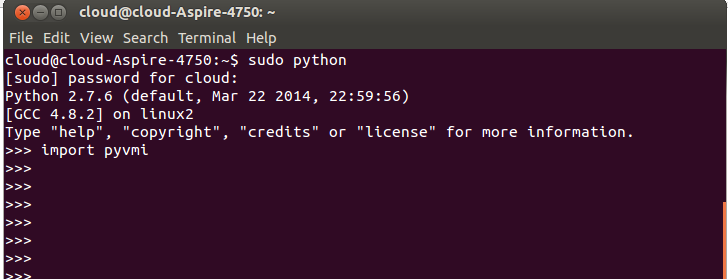
\includegraphics[width=14cm, height= 10cm ]{Figures/Figure22.png}
	\caption[Import Pyvmi in Python interactive Shell]{Import Pyvmi in Python interactive Shell}
	\label{fig:Import Pyvmi in Python interactive Shell}
\end{figure}

Run python in a terminal and try to import pyvmi module, nothing output means that LibVMI has been encapsulated as module into Python. 
Now we could invoke LibVMI API in Python script.

Now it’s time to get Volatility.
\shellcmd {cd ~/libvmi}
\shellcmd {wget https://volatility.googlecode.com/files/volatility-2.3.tar.gz}
\shellcmd{tar zxvf volatility-2.3.tar.gz}
\shellcmd{cd volatility-2.3.tar.gz}

In term of installing Volatility's code, we have two choices, each has its own advantages and disadvantages.

1) Extract the archive and run setup.py. This way is useful when we want to import Volatility as module in Python script, however, it is not 
convenient for upgrading or uninstalling.


2) Extract the archive to a directory of your choice. When you want to use Volatility just do python /path/to/directory/vol.py. This is a 
cleaner method since no files are ever moved outside of your chosen directory, which is convenient for possible update of Volatility in the 
future. The cost is that Volatility could not be used as a library in Python script.

For our case, we choose to run setup.py for the purpose of using Volatility as a module. Now we manage to install LibVMI and Volatility in 
our KVM experimentation platform. The following section will talk about my manipulation.

\section{Explore Volatility with LibVMI}
This section is used to record the exploration course of exploring the usage of Volatility and LibVMI for running KVM virtual machines. 
The first section is about a general introduction about Volatility.
\subsection{Introduction about Volatility}
The Volatility Framework is a completely open-source collection of tools, implemented in Python under the GNU General Public License, 
for the extraction of digital artifacts from volatile memory (RAM) samples. The extraction techniques are performed completely independent 
of the system being investigated but offer visibility into the runtime state of the system. The framework is intended to introduce people 
to the techniques and complexities associated with extracting digital artifacts from volatile memory samples and provide a platform for 
further work into this exciting area of research. The official documentation is very complete and is available here
: \url{http://code.google.com/p/volatility/wiki/VolatilityIntroduction?tm=6}.
\subsection{Volatility Usage}
Since the installation is introduced previously, here we talk about directly the usage of this powerful tool. Briefly, the most basic 
volatility commands are constructed as shown below:
\shellcmd{python path/to/vol.py [plugin] -f [image] --profile=[profile]}
Placeholder [plugin] in above command line represents the functionality provided by Volatility. For example “pslist” plugin allows listing all 
currently running processes. [image] means the path to the target memory dump. It could be in various types depending supported address 
space, such as raw dd style format or LiME \cite{Reference35} format for Linux. [profile] indicates which memory layout or kernel data structure will 
be used to investigate input memory sample file. One reason why Volatility is so useful and popular is due to complete and predefined 
profile for Windows.

Replace plugin with the name of the plugin to use (pslist, netscan, linxu\_netstat,etc.), image with the file path to your memory image, 
and profile with the name of the profile (such as Win7SP1x64, the default profile is always WinXPSP3x86).

For example, imaging a Windows guest memory dump named “win7.dd” is at our disposal. Now we want to investigate which network connections are established.  
The following command is used to achieve this:
\shellcmd{sudo python vol.py netscan -f /path/to/win7.dd –profile=Win7SP1x86}
For everything beyond this example, such as controlling the output format, listing the available plugins and profiles, or supplying 
plugin-specific options, see the rest of the text below. https://code.google.com/p/volatility/wiki/VolatilityUsage23


\subsection{Plugin}
As mentioned above, the functionalities of Volatility are in implemented in form of plugin and could be extended. Initially, 
Volatility is used uniquely for Windows memory analysis, thus it provides up to now variety of plugins for Windows. This plugins could 
be grouped into the those categories shown in Figure \ref{fig:Windows Core Plugin List}:

\begin{figure}[htbp]
	\centering
		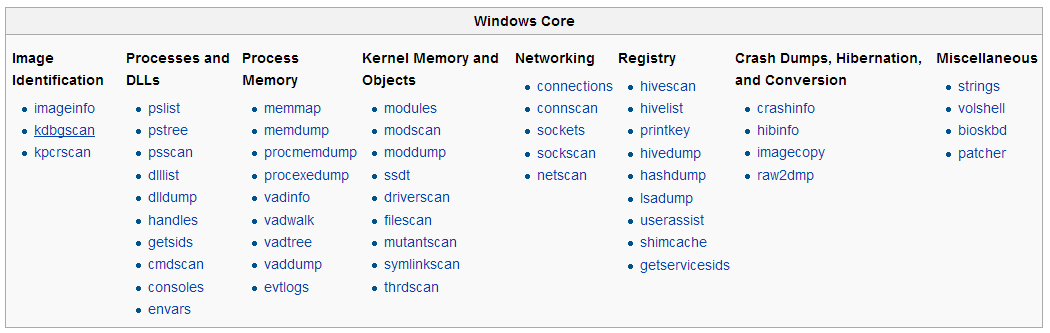
\includegraphics[width=14cm, height= 10cm ]{Figures/Figure23.png}
	\caption[Windows Core Plugin List]{Windows Core Plugin List \cite{Reference13}}
	\label{fig:Windows Core Plugin List}
\end{figure}

Thus with Volatility, we could get a rather clear visibility for the security or monitoring purpose, for the running state of the target
machine if we have its memory sample file.

\begin{figure}[htbp]
	\centering
		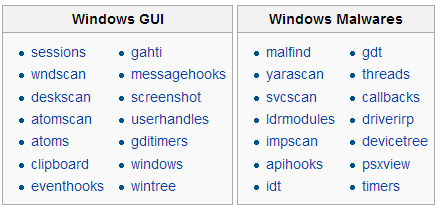
\includegraphics[width=14cm, height= 10cm ]{Figures/Figure24.png}
	\caption[Windows GUI and Malware Plugins List]{Windows GUI and Malware Plugins List \cite{Reference13}}
	\label{fig:Windows GUI and Malware Plugins List}
\end{figure}

Before Volatility version 2.1, Volatility does not support memory forensic analysis for Linux. At the moment, another FMA tool called 
Volitilinux is used for this task. Volitilinux could be regarded as counterpart of Volatility for Linux. From Volatility version 2.2, 
Volatility has incorporated Volitlinux’s functionality and has a more wide range OS support.

In term of Linux, available plugins are resumed in Figure \ref{fig:Linux Memory Forensic Plugin}.
\begin{figure}[htbp]
	\centering
		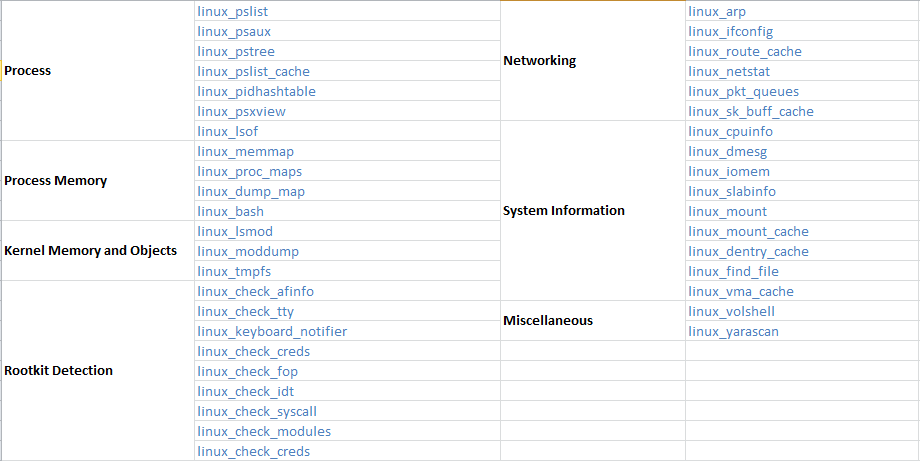
\includegraphics[width=14cm, height= 10cm ]{Figures/Figure25.png}
	\caption[Linux Memory Forensic Plugin]{Linux Memory Forensic Plugin \cite{Reference36}}
	\label{fig:Linux Memory Forensic Plugin}
\end{figure}

In this article, we will not present all the available plugins.
Here we pick up some typical and useful command to present the power of Volatility. 
For example, Figure \ref{fig:Volatility netscan(for windows) plugin's output} demonstrates that “netscan” command helps us to get all 
the currently established network connections with their corresponding process.

\begin{figure}[htbp]
	\centering
		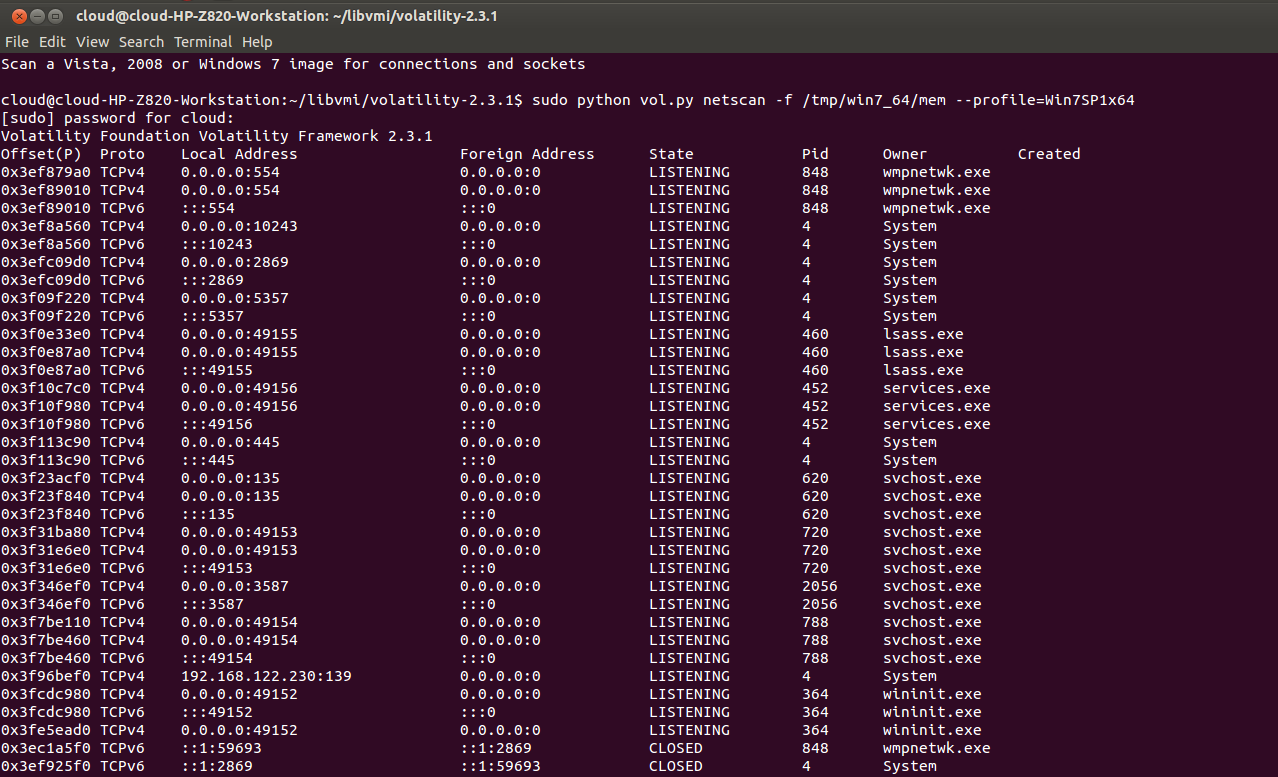
\includegraphics[width=14cm, height= 10cm ]{Figures/Figure26.png}
	\caption[Volatility netscan(for windows) plugin's output]{Volatility netscan(for windows) plugin's output}
	\label{fig:Volatility netscan(for windows) plugin's output}
\end{figure}

Up to now, the actual list of available plugins is long and grows quickly due to the strong development community. 
We could leverage these plugins to develop our own VMI applications or extend the list of available plugins.

\subsection{Profile}
Volatility is actually an out-of-band method to mitigate the semantic gap, due to the fact that before executing forensic memory, 
some configuration files about operating system kernel data structures are required. 
This kind of configuration file is usually called “Profile”. 
The command “sudo python path/to/vol.py --info | grep -i Profile” returns the profile list 
(Figure \ref{fig:Supported Profile List in Our KVM Platform})currently supported by Volatility.

\begin{figure}[htbp]
	\centering
		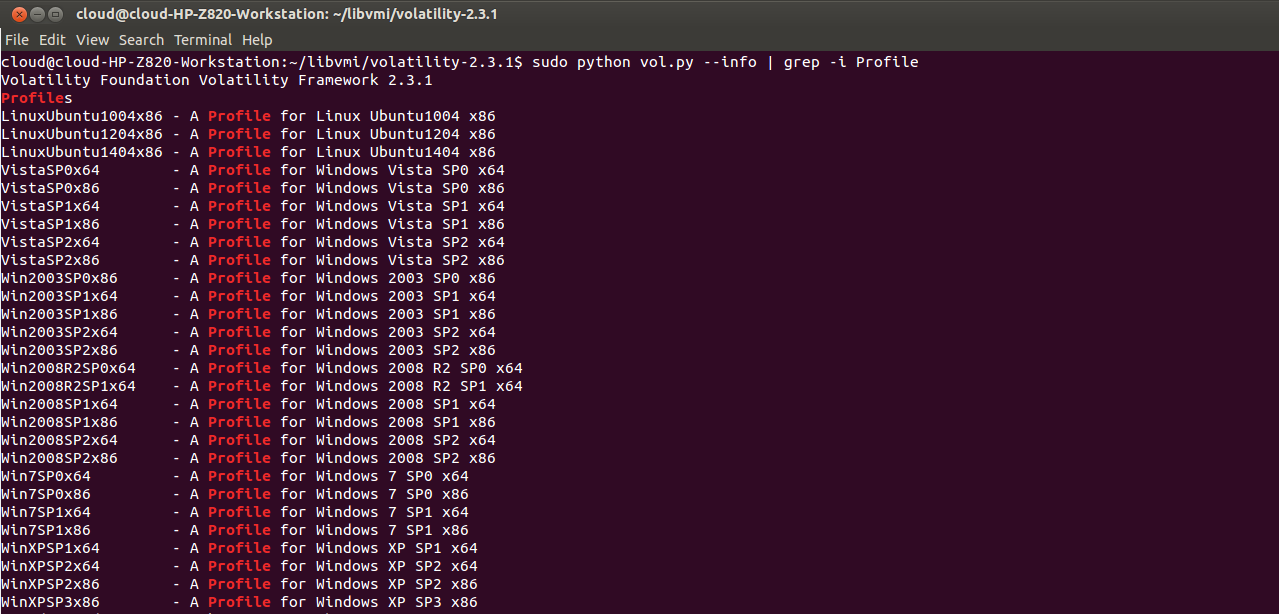
\includegraphics[width=14cm, height= 10cm ]{Figures/Figure27.png}
	\caption[Supported Profile List in Our KVM Platform]{Supported Profile List in Our KVM Platform}
	\label{fig:Supported Profile List in Our KVM Platform}
\end{figure}

Those who need an attention is, Volatility by default has provided profiles for all existing Windows series OS, 
because Windows OS’s kernel versions are relatively stable. For Windows guest memory analysis, no additional steps are necessary to 
generate the corresponding profile. This is not the case for Linux. Since there exists all kinds of Linux distribution and Linux’s 
kernel is always in constant evolution, we need to create a unique profile for every kernel version (2.6.x, 3.x, etc.), every 
distribution (such as Ubuntu/Fedora/CentOS,etc.). Plenty of online tutorials are available for this subject, for example: 
\url{https://code.google.com/p/volatility/wiki/LinuxMemoryForensics}.

\subsection{Address Space}
The address space notion is used to describe different memory dump. 
For different memory dump format, corresponding address space should be used to assure the correct functioning of memory analysis. 
It’s not necessary to indicate which address space is used when calling a certain Volatility command. 
Volatility applies a heuristic algorithm to automatically choose the appropriate address space for input memory dump. 
The following figure has shown all support address space in our KVM virtualization platform.

\begin{figure}[htbp]
	\centering
		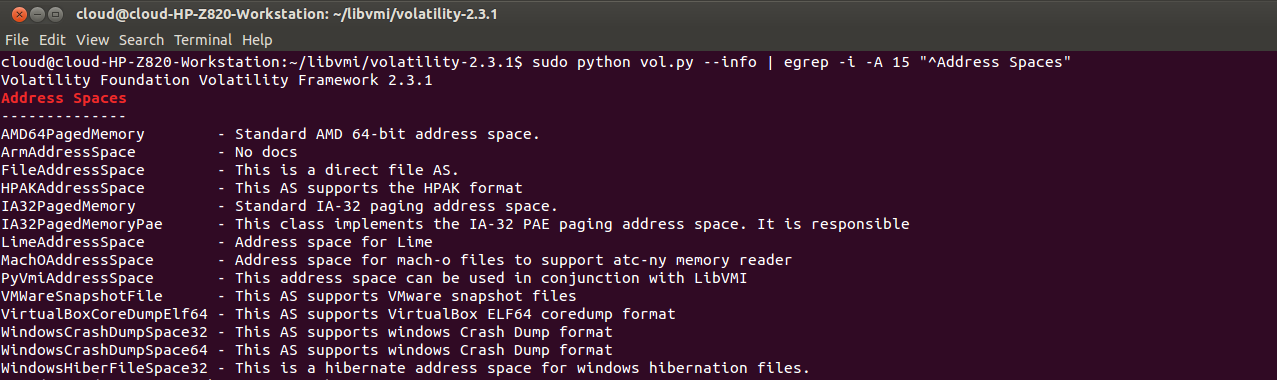
\includegraphics[width=14cm, height= 7cm ]{Figures/Figure28.png}
	\caption[Volatility Supported Address Space]{Volatility Supported Address Space}
	\label{fig:Volatility Supported Address Space}
\end{figure}

The address space could be also extended by developing special plugin for special memory dump. 
For example, to make Volatility to support LibVMI’s API, the author of LibVMi has developed a special address space plugin called 
“PyVmiAddressSpace”. It’s only necessary to copy Python script “pyvmiaddressspace.py” into the following directory under 
Volatility 2.3: volatility/plugins/addrspaces/.

\section{Cooperation with LibVMI}
Volatility is designed to work on forensic memory snapshots. In this mode, a forensic analyst would take a physical memory image from
a target machine, and then use Volatility to extract useful information from that image. However, since Volatility already contains 
significant information on the Windows/Linux memory layout and because Volatility greatly simplifies the development of memory analysis 
tools, LibVMI development team tried to integrate Volatility with LibVMI to facilitate analysis on a running virtual machine \cite{Reference8}. Thanks
to their great job, now a “VMI application-LibVMI-Volatility” tool chain has been established to simplify the development of VMI application.
In this section, we talk about how they make Volatility work directly on a live virtual machine.

In fact, LibVMI is implemented in C and we should develop some VMI applications (out-of-band) with its C library. With the popularity of 
Python in VMI research domain, LibVMI also provides a Python wrapper called PyVMI to allow LibVMI being used by Python script, such as 
Volatility framework. Their effort has formed the software stack shown in Figure \ref{fig:Software stack with PyVMI wrapper on top of the C language LibVMI library}.

\begin{figure}[htbp]
	\centering
		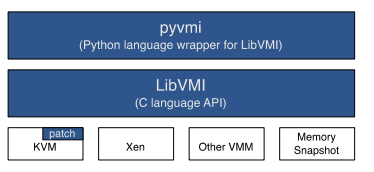
\includegraphics[width=14cm, height= 7cm ]{Figures/Figure29.png}
	\caption[Software stack with PyVMI wrapper on top of the C language LibVMI library]
	{Software stack with PyVMI wrapper on top of the C language LibVMI library \cite{Reference6}}
	\label{fig:Software stack with PyVMI wrapper on top of the C language LibVMI library}
\end{figure}

With Pyvmi, LibVMI could be used a module in Python script. Now, we should consider how to allow Volatility functioning on a live virtual machine. 
To do this, LibVMI provides two mechanisms.

\subsection{PyVMI Address Space Plugin}
This first mechanism is using a special address space plugin called “PyVMIAddressSpace”. Figure \ref{fig:Software stack with Volatility address space plugin}
shows how Volatility plugins could leverage this address space plugin to cooperate with LibVMI. Supposing we want to investigate which 
processes are currently running in target guest named “win7\_32bit”, this command could help us:
\shellcmd{sudo python path/to/vol.py pslist -l vmi:///win7\_32bit --profile=Win7SP1x86}
Although LibVMI development team announced that with PyVMI address space plugin, all Volatility plugins will work on a running virtual 
machine. With my manipulation we encountered some unexpected problems. Firstly, this plugin works for almost all Windows plugin while 
plants for some Linux plugins such as linux\_netstat. Secondly, sometimes (not always) after applying for example netscan plugin for a 
Windows, I found that the volume of log file (under path /var/log/libvirt/qemu) possibly augmented until all root file system’s disk 
space was all consumed. To solve this problem, I have posed this problem in LibVMI google discussion group but not received any response. 
I don’t know this problem is specific to my KVM platform. Therefore, at least in my work environment, PyVMI address space plugin is not 
recommended compared to its alternative.

\begin{figure}[htbp]
	\centering
		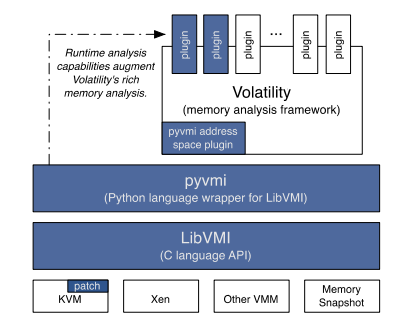
\includegraphics[width=14cm, height= 9cm ]{Figures/Figure30.png}
	\caption[Software stack with Volatility address space plugin]{Software stack with Volatility address space plugin \cite{Reference6}}
	\label{fig:Software stack with Volatility address space plugin}
\end{figure}

\subsection{Pyvmifs.py script}
The second mechanism is firstly mounting virtual machine’s physical memory as a regular file then using Volatility to analyze this 
memory file as if it were static. LibVMI has provided a special Python script to achieve this task. Its usage is:
\shellcmd{sudo python path/to/pyvmifs.py -o allow\_other -o domain=GUEST\_NAME path/to/mount/point}
Still take our Windows guest “win7\_32bit” as example. After above invocation, its physical memory is mounted under path 
/tmp/win7\_32bit/mem. Then invoke for example pslist plugin to get the running process list:
\shellcmd{sudo python path/to/vol/py pslist -f /tmp/win7\_32bit/mem --profile=Win7SP1x86}
Different with pyvmi address space plugin, the simple Python script works well and poses none problem.

\section{Experimentation Result}
With LibVMI+pyvmifs.py+volatility, we could run all interesting plugins for our KVM Windows/Linux virtual machines. 
Figure shows the resume of execution of under Windows 7 x86/64 and Ubuntu 10.04 x86.

\begin{figure}[htbp]
	\centering
		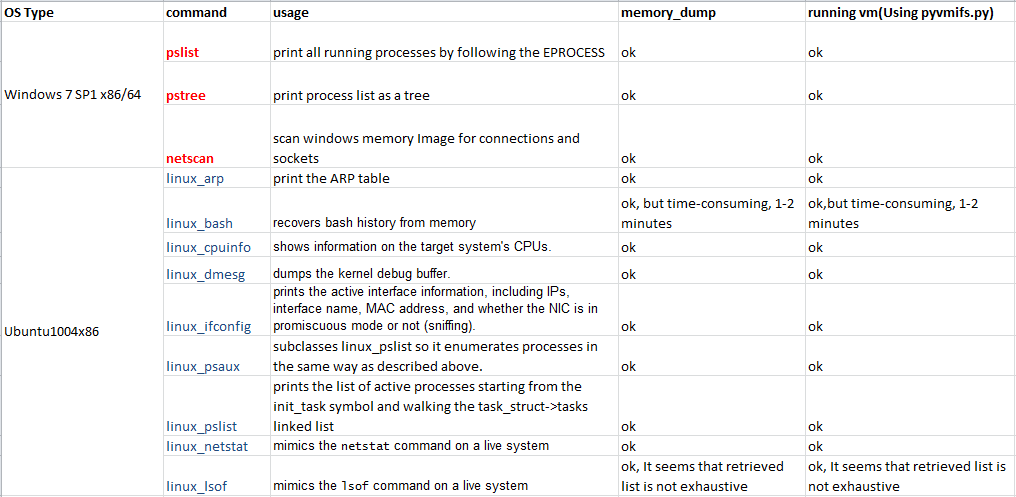
\includegraphics[width=14cm, height= 9cm ]{Figures/Figure31.png}
	\caption[Experimentation Result of Volatility Plugins in KVM Platform]{Experimentation Result of Volatility Plugins in KVM Platform}
	\label{fig:Experimentation Result of Volatility Plugins in KVM Platform}
\end{figure}

7.7Limit of Volatility\&LibVMI

Although Volatility presents various advantages in memory forensic analysis domain, its disadvantages are still obvious in the context 
of Virtual Machine Introspection: Volatility is applied uniquely to memory analysis, whereas Virtual Machine Introspection could also 
cover introspection on virtual CPU or virtual disk. Fortunately, LibVMI and libguestfs \cite{Reference38} could come to cover this shortage. 
LibVMI allows monitoring the running state of vCPU and libguestfs library is able to access and modify virtual machine’s disk image. 







